%!TEX root = ../thesis.tex

\section{Conclusion}
\label{sec:conclusion}

In this section, we will give a final summary of our work, draw conclusion in light of the requirements towards verification of specifications against higher level properties that were imposed both by us and \citeauthor{Reid17} in \cite{Reid17} and give an outlook for possible future work.
Find an overview of this thesis as a whole in figure \ref{fig:overview}.
As a first step we developed the MINRV8 architecture in section \ref{sec:model} that was inspired by the \gls{riscv} architecture and implemented in \gls{nuxmv}.
In section \ref{sec:checking}, we developed information flow semantics and three information flow properties forming an information flow policy in spirit of the work of \citeauthor{Ferraiuolo17} \cite{Ferraiuolo17}.
The information flow semantics were used to augmented the model of the MINRV8 by information flow tracking.
In section \ref{sec:results} we introduced eight assumptions that, when implemented software running in machine-mode such as \glspl{os}, guarantee the absence of vulnerabilities covered by aforementioned information flow properties.
We evaluated our model, the properties and the assumptions by showing that taken together, they manage to detect both the cache poisoning \cite{Wojtczuk09} and the SYSRET vulnerability \cite{Dunlap19}.
Finally in section \ref{sec:discussion}, we discussed the limitations and the scope of our work and reflected whether our methodology is trustworthy.

\begin{figure}
    \centering
    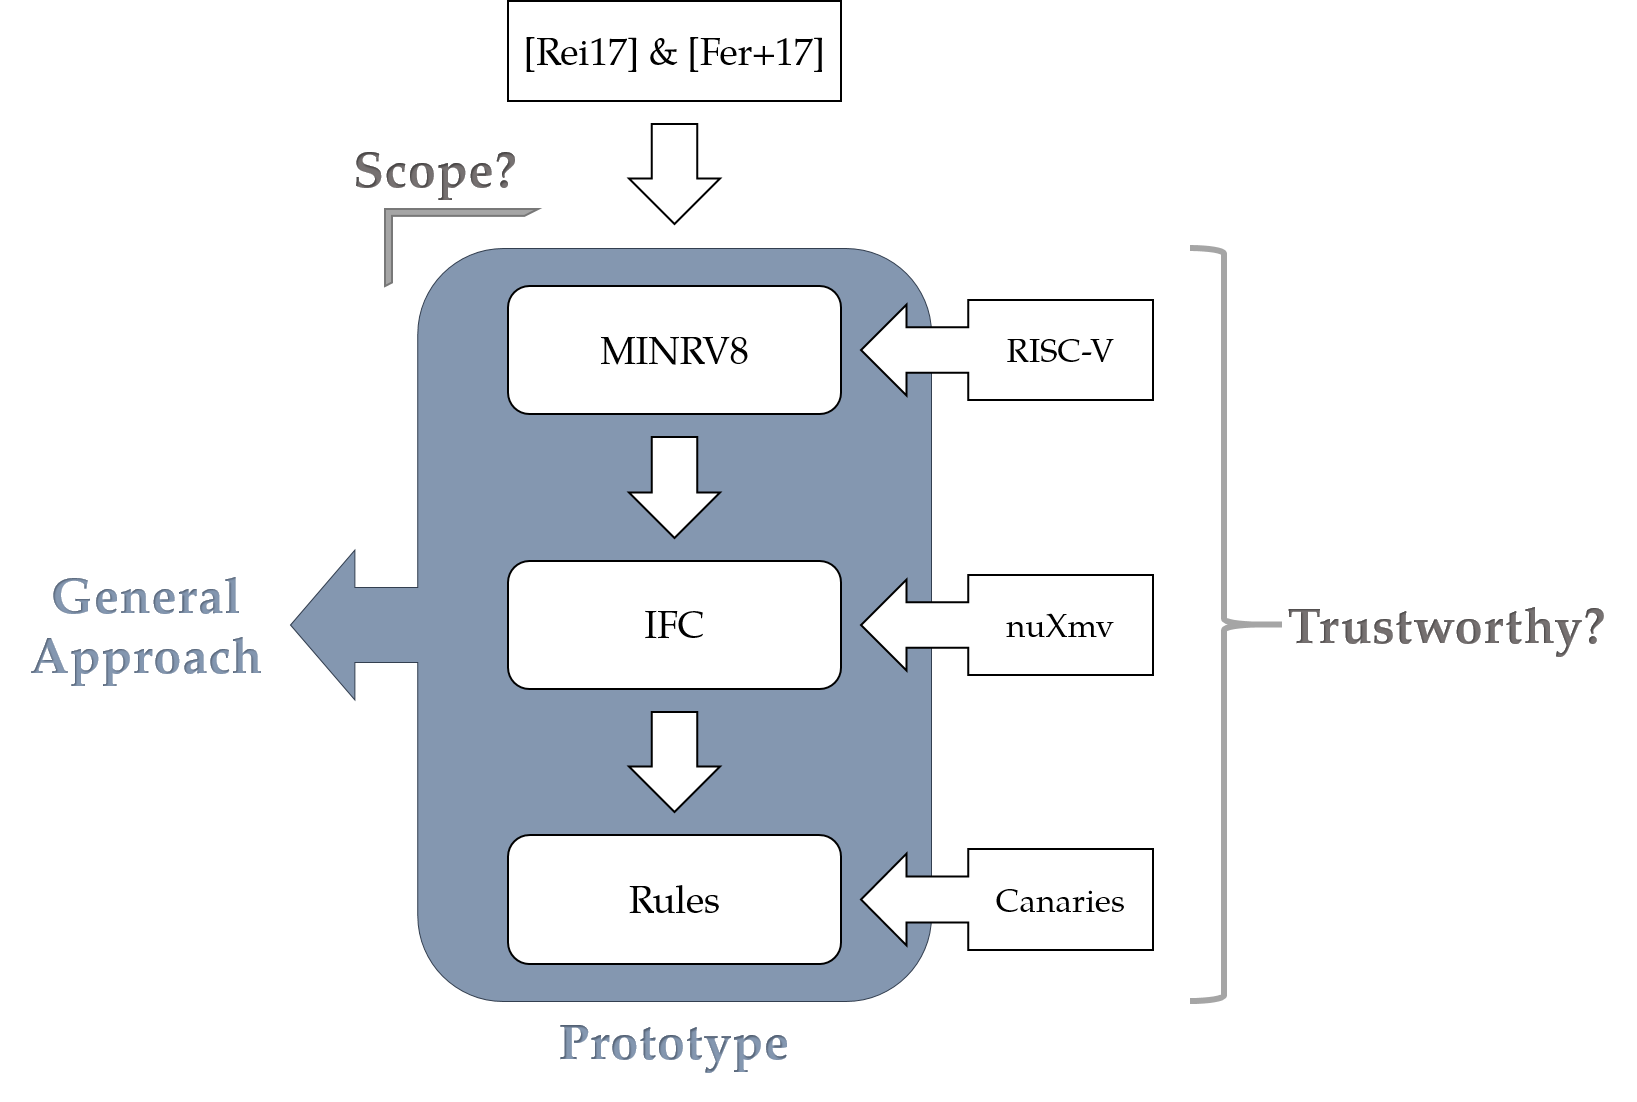
\includegraphics[width=\textwidth]{figures/thesis-overview.png}
    \caption{Thesis Overview}
    \label{fig:overview}
\end{figure}
